\chapter{Stand der Wissenschaft und Auswahl von Verfahren}

In diesem Kapitel soll der aktuelle Stand der Wissenschaft\todo{Naja SIEM eher weniger Wissenschaft} bezogen auf die in dieser Arbeit verwendeten Klassen von Verfahren betrachtet werden sowie ausgehend von den Anforderungen an das zu entwickelnde System ein passendes Verfahren ausgewählt und im Detail beschrieben werden. An geeigneten Stellen wird auf die im letzten Kapitel dargelegten Grundlagen zurückgegriffen.

\todo{Vielleicht als Übergang eine ein bisschen ausführlichere Beschreibung des Systems, um das Zusammenspiel der verschiedenen Verfahren besser zu verstehen? Dieser Teil könnte dann in der Einführung mit Verweis kürzer ausfallen.}

\label{cha_state}

\section{SIEM-Systeme}

\label{sec_state_siem}

Zur Zeit gibt es eine vielfältige Auswahl an SIEM-Systemen auf dem Markt, die die grundsätzlichen Aufgaben eines SIEM-Systems erfüllen und über diese hinausgehen: Splunk\footnote{
  https://www.splunk.com
}, QRadar von IBM\footnote{
  https://www.ibm.com/us-en/marketplace/ibm-qradar-siem
} oder ArcSight von Micro Focus\footnote{
  https://software.microfocus.com/en-us/software/siem-security-information-event-management
} sind nur einige Beispiele aus diesem Bereich. \todo{Die Funktionen dieser Systeme sind alle ähnlich/total unterschiedlich/ gehen von bis usw.}

\todo{Umschreiben - OSSIM weil ...}

Die Auswahl an Open-Source-Software in diesem Bereich ist jedoch sehr gering. Eine der wenigen Ausnahmen stellt OSSIM - ein SIEM-System der Firma AlienVault\footnote{
	AlienVault OSSIM: The World’s Most Widely Used Open Source SIEM\\https://www.alienvault.com/products/ossim
} - dar, das auf Basis weiterer quelloffener Lösungen aus dem Netzwerksicherheits-Bereich unter anderem die in Abschnitt \ref{sec_basics_siem} beschriebenen Funktionen bereitstellt. AlienVault bietet zusätzliche eine kommerzielle Variante seines Produkts namens USM an, das insbesondere in den Bereichen Event-Korrelation und Compliance-Reporting die Funktionalität von OSSIM übersteigt. Von der Entwicklungsarbeit die in USM fließt, profitiert jedoch auch OSSIM, beispielsweise durch die Aktualisierung von Plugins für die Einbindung von aktuellen Netzwerkgeräten.

\subsection{OSSIM-Überblick}

\label{subsec_state_siem_overview}

Im Folgenden soll eine Übersicht über die für diese Arbeit relevanten Komponenten von OSSIM und deren Zusammenspiel gegeben werden. Diese ist auch in Abbildung \ref{fig:ossim_log_flow} dargestellt.

Den Kern des SIEM-Systems bildet der OSSIM-Server. Hier werden Events gespeichert sowie aggregiert und es findet die Korrelation von Events statt, die der Erkennung von Angriffen oder ungewöhnlichem Netzverhalten dient. Events und generierte Meldungen können über ein Web Interface betrachtet werden. Weiterhin können hier unter anderem Angaben zur Netzinfrastruktur bereitgestellt, Netzwerk- und Schwachstellenscanner bedient und sämtliche Informationen über den Netzwerkstatus eingesehen werden. 

Der OSSIM-Agent ist dafür zuständig, vorliegende Logdaten zu parsen und in ein OSSIM-spezifisches Event-Format zu übersetzen. Auf diesen Vorgang wird im nächsten Abschnitt genauer eingegangen. Die erzeugten Events werden anschließend an den Server weitergeleitet. Der Agent befindet sich sowohl direkt auf dem Server als auch auf jedem installierten Sensor. 

Eine OSSIM-Umgebung kann optional ein oder mehrere Sensoren nutzen, auf denen jeweils ein Agent seine Arbeit verrichtet. Dies wird im Folgenden verteilte Installation genannt. Der Vorteil dieser Lösung besteht darin, dass das aufwendige Parsen und Normalisieren von Logdaten verteilt staffinden und dadurch die Serverlast in großen Umgebungen reduziert werden kann. Kommt kein externer Sensor zum Einsatz, so spricht man von einer All-In-One-Installation.

\begin{figure}[]
    \centering
        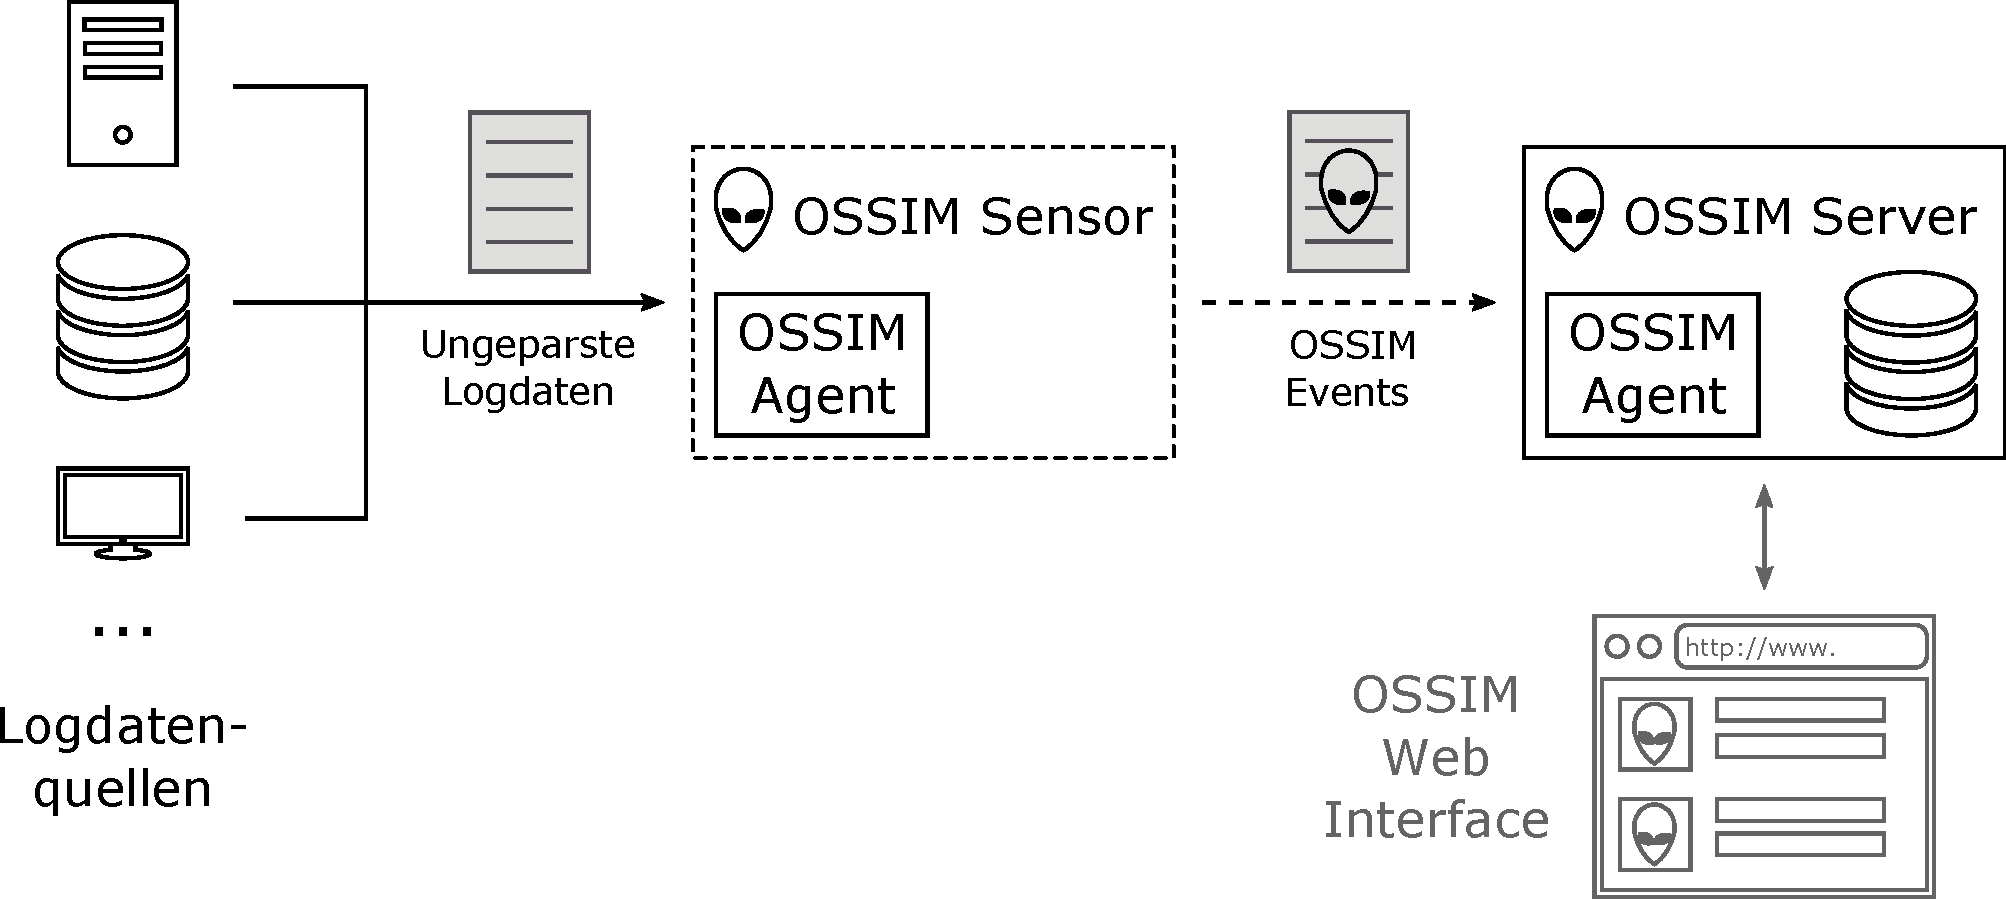
\includegraphics[width=0.9\textwidth]{dia/ossim_log_flow.pdf}
    \caption{High-Level-Übersicht über die OSSIM-Architektur und den Datenfluss.}
    \label{fig:ossim_log_flow}
\end{figure}


\subsection{Parsen von Logdaten in OSSIM}

\label{subsec_state_siem_parsing}

% Quellenarten
% Plugins
% OSSIM-Events
Besonders von Bedeutung für diese Arbeit ist die Verarbeitung von Logdaten. OSSIM ermöglicht es, Logdaten aus unterschiedlichen Quellen entgegenzunehmen bzw. aktiv selber abzurufen und in ein gemeinsames Event-Format zu übersetzen. Hierzu stehen verschiedene Möglichkeiten zur Verfügung:

\begin{itemize}
  \item Entgegennehmen von Daten über das Syslog-Protokoll
  \item Beschaffen von Daten über das SNMP-Protokoll
  \item Entgegennehmen von Daten über proprietäre Protokoll wie SDEE oder WMI
  \item Beschaffen von Daten durch Datenbankabfragen 
\end{itemize}

Unabhängig von der Datenquelle funktioniert die Verarbeitung der Logdaten nach dem immer gleichen Schema. OSSIM bietet die Möglichkeit mitgelieferte oder selber entwickelte Plugins für verschiedene Datenquellen zu aktivieren. Für eintreffende Logdaten überprüft der Agent anhand von regulären Audrücken, ob ein Plugin für das entsprechende Datum zuständig ist. Ist so ein Plugin gefunden, so wird ein neues OSSIM-Event angelegt und anhand der Angaben im Plugin die entsprechenden vorgegebenen Felder des Events gesetzt. Hierbei kann es sich beispielsweise um den Zeitpunkt des Events, IP-Adresse und Port der Datenquelle, einen zu dem Event gehörigen Netzwerkbenutzer oder ereignisabhängige selbstgesetzte Felder handeln. Anschließend folgt die Weiterleitung des Events an den Server.


\section{Pseudonymisierung}

\label{sec_state_pseudonymity}

%pfitzmann2001 - Abschnitt 12
Der Begriff der Pseudonymisierung beschreibt die Benutzung von Pseudonymen zur Identifizierung von Subjekten. Ein Pseudonym (im technischen Sinne) kann nach \cite{pfitzmann2010} als einfache Bitkette betrachtet werden. Es sollte zufällig generiert werden, d.h. vollkommen unabhängig von dem zugehörigen Subjekt oder es betreffenden Eigenschaften sein, um keine Rückschlüsse aus dem Pseudonym selbst zu ermöglichen. Ein Negativbeispiel wäre ein nutzervergebenes Pseudonym, das den Namen des Haustiers enthält. Aber beispielsweise auch eine aufsteigende Nummerierung als Pseudonym könnte durch den hierdurch genauer spezifizierten Erstellungszeitpunkt Rückschlüsse auf das Subjekt hinter dem Pseudonym ermöglichen.

Pseudonymisierung sagt erst einmal lediglich etwas über die Verwendung eines Verfahrens aus, jedoch nichts über die daraus entstehenden Auswirkungen auf die Identifizierbarkeit eines Subjekts oder die Zurechenbarkeit bestimmter Aktionen. Hierfür spielen nach \cite{pfitzmann2001} weitere Eigenschaften von Pseudonymen wie die folgenden eine Rolle:
\begin{itemize}
  \item garantierte Eindeutigkeit von Pseudonymen
  \item Möglichkeit von Pseudonymänderungen
  \item begrenzt häufige Verwendung von Pseudonymen 
  \item zeitlich begrenzte Verwendung von Pseudonymen
  \item Art der Pseudonymserstellung
\end{itemize}

Um die Auswirkungen dieser Eigenschaften einordnen zu können, soll im Folgenden kurz die Pseudonymisierung in zwei Systemen betrachtet und die Relevanz der eben genannten Eigenschaften verdeutlicht werden: Pseudonyme in Mobilfunknetzen und in der Fahrzeug-zu-Fahrzeug-Kommunikation. 

\subsection{Mobilfunknetze}

In Mobilfunknetzen wird zur Identifikation eines Teilnehmers anstelle seiner identifizierenden \textit{International Mobile Subscriber Identity} meist ein Pseudonym -- die \textit{Temporary Mobile Subscriber Identity} (TMSI) -- genutzt, das in bestimmten Situationen gewechselt wird und so Ortung und Bewegungsprofile der Teilnehmer verhindern soll.
In \cite{arapinis2014} beschreiben die Autoren Schwächen der Implementierungen von Mobilfunkstandards in Netzen bei der (Neu-)Vergabe einer TIMSI. Bestimmte Eigenschaften im Bezug auf die Unverkettbarkeit von Pseudonymen und damit auf die Privatsphäre der Nutzer werden in vielen Netzen aufgrund einiger Schwächen nicht erreicht:
\begin{itemize}
  \item Zu seltene Änderung der Pseudonyme
  \item Keine nutzungsabhängige Änderung von Pseudonymen
  \item Pseudonyme werden in verschiedenen Bereichen beibehalten
  \item Anfälligkeit der Neuvergabe für Replay-Angriffe
\end{itemize}
Die letzten beiden Schwächen sind für den Anwendungskontext dieser Arbeit nicht relevant, aber die zeit- und aktivitätsabhängige Neuvergabe von Pseudonymen müssen auch hier beachtet und umgesetzt werden.

\subsection{VANets}

Ein anderer Bereich, der sich besonders mit der Nutzung von Pseudonymen beschäftigt hat, ist die Forschung an Vehicular Ad Hoc Networks (VANets). Hierbei handelt es sich um Netzwerke für die Kommunikation zwischen Fahrzeugen, die beispielweise für die Datenübermittlung zur Bremserkennung naher Fahrzeuge oder die Stauerkennung genutzt werden können. Um die Privatsphäre der Fahrzeughalter zu schützen, wird für die Kommunikation in vielen Ansätzen auf die Verwendung von Pseudonymen gesetzt. So soll sich beispielsweise das Anlegen von Bewegungsprofilen verhindern lassen.\\
Unter anderem in \cite{dotzer2005} und \cite{petit2015} widmen sich die Autoren der Nutzung von Pseudonymen in VANets und den besonderen Anforderungen, die diese erfüllen müssen -- insbesondere auch im Hinblick auf die Häufigkeit von Pseudonymwechseln. Es ergibt sich, dass die Häufigkeit und Situation\footnote{
  Es werden beispielweise Lösungen vorgestellt, die abhängig von Geschwindigkeitsänderungen, einer gewissen Anzahl anderer Fahrzeuge oder besonderen Verkehrssituationen wie Kreuzungen die Pseudonymänderung vornehmen. Das Ziel ist hier immer die Möglichkeit der Pseudonymverkettung bzw. der Bewegungsprofilerstellung durch die äußere Situation der Pseudonymänderung zu erschweren.
}, in der Pseudonymwechsel stattfinden sollten, abhängig vom gewünschten Grad an Anonymität bzw. Angreifermodell sind und außerdem gegenüber Sicherheitsanwendungen\footnote{
  Beispielsweise wäre zur VANet-basierten Kollisionsvermeidung eine Verkettung von Orten, an denen sich ein Fahrzeug zu verschiedenen Zeitpunkten befindet, erstrebenswert.
}  abgewogen werden müssen.\\
Bei der Nutzung von Pseudonymen in VANets handelt es sich natürlich um eine Anwendung mit anders gelagerten Prioritäten im Vergleich zu dem Kontext dieser Arbeit. Dennoch wird deutlich, dass die Strategie zum Pseudonymwechsel stark von der Anwendungssituation abhängig ist. Bezogen auf den hier vorliegenden Anwendungsfall werden insbesondere Besonderheiten der Datenquelle, wie die Häufigkeit von auftretenden Überwachungsdaten, und Anforderungen an die Verknüpfbarkeit von Ereignissen der auf den Daten beruhenden Anomalieerkennung zu beachten sein.

% Perfect Forward Privacy

In \cite{schaub2009} stellt der Autor eine weitere Anforderung an die Nutzung von Pseudonymen in VANets, die jedoch nicht nur für diesen speziellen Anwendungsfall relevant ist: Er verlangt, dass die Aufdeckung eines Pseudonyms keine Informationen über die Identität eines Nutzers im Bezug auf andere Pseudonyme ermöglichen sollte. Diese Eigenschaft bezeichnet er als \textit{Perfect Forward Privacy}\footnote{
  Die Bezeichnung ist an \textit{Perfect Forward Secrecy} angelehnt. Diese Eigenschaft beschreibt ein ähnliches Verhalten bei der verschlüsselten Kommunikation: Ein Angreifer, der in den Besitz des Langzeitschlüssels eines Kommunikationspartners kommt, sollte trotzdem nicht in der Lage sein, bereits aufgezeichnete Nachrichten entschlüsseln zu können.
}.

\subsection{Pseudonymisierung im zu entwickelnden System}

% - Pseudonymgenerierung
% - Pseudonymwechsel zeit und datenmengenabhängig
%   leider nicht genauer, da sowohl datenquellen als auch anomaliedings nicht klar
%   daher parameter ermöglichen
% - PFP in DB umsetzen

Aus diesen Vorüberlegungen können nun die Rahmenbedingungen der in dieser Arbeit verwendeten Pseudonymisierung aufgestellt werden.
Pseudonyme sollten als zufällig gewählte Bitketten hinreichender Länge gewählt werden. Ihre Eindeutigkeit muss sichergestellt werden.

Wie auch in den Beispielen deutlich wurde, müssen Pseudonyme abhängig von dem Anwendungsszenario in bestimmten Fällen für einen Benutzer gewechselt werden. In dem hier vorliegenden Anwendungsfall, in dem Pseudonyme für die Zuordnung von eintreffenden Überwachungsdaten in Unternehmensnetzen genutzt werden, sind insbesondere die Zeitabhängigkeit sowie die Abhängigkeit von der Nutzungshäufigkeit für die Pseudonymwechselstrategie ausschlaggebend. Verschiedene Nutzeraktionen sollten nur in einem gewissen zeitlichen Rahmen und nur in einer gewissen Häufigkeit verkettbar sein. Es handelt sich also um eine schwächere Form der Transaktionspseudonyme, bei der ein Pseudonym je nach Pseudonymwechselstrategie nur für eine bestimmte Anzahl an Ereignissen verwendet wird.

Eine über diese generelle Aussage hinausgehende Bewertung davon, wie diese Abhängigkeiten konkret zu implementieren sind, ist jedoch im Rahmen dieser Arbeit nicht zu leisten. Hierfür sind zwei Gründe ausschlaggebend:
\begin{itemize}
  \item Sie hängen stark von den Eigenschaften der Datenquellen ab, die die Überwachungsdaten liefern. Beispielsweise wäre das Datenprofil, das von einem elektrischen Türschließsystem geliefert wird, sehr unterschiedlich zu dem, das Zugriffe auf einen Netzwerkspeicher protokolliert. Im ersten Fall würden im Allgemeinen selten Daten anfallen, die zudem durch die Anwendung von Hintergrundwissen (Benutzer wird beim Betreten eines Raumes beobachtet) eher zur Aufdeckung eines Pseudonyms führen könnten. Hier wären wahrscheinlich häufige nutzungsabhängige Wechsel angebracht. Eventuell wäre sogar der Extremfall einer einmaligen Pseudonymvergabe pro Aktion in Erwägung zu ziehen.\\
  Im zweiten Fall hingegen würden im Allgemeinen häufig Daten anfallen und erst die Verkettung dieser Daten könnte hilfreiche Rückschlüsse auf vorliegende Anomalien liefern. Ein einzelner Datenzugriff hätte meist wenig Aussagekraft, wohingegen ein massenhafter Zugriff beispielsweise auf die Kundendatenbank eines Unternehmens durch einen gekündigten Mitarbeiter möglicherweise auf Datendiebstahl schließen lassen könnte.
  
  \item Weiterhin muss die Pseudonymwechselstrategie auch abhängig von der später auf den pseudonymisierten Überwachungsdaten auszuführenden automatisierten Anomalieerkennung sein. Je nachdem welche Verfahren auf Daten aus welchen Datenquellen eingesetzt werden sollen, könnte auch hier unterschiedliche Verknüpfbarkeit der Daten erforderlich sein. Hieraus ergibt sich auch ein Spannungsfeld zwischen den Anforderungen der Anomalieerkennung gegenüber der Verknüpfbarkeit der Daten und damit der Privatsphäre der Arbeitnehmer.
\end{itemize}

Aus diesen Gründen wird eine parameterabhängige Pseudonymwechselstrategie implementiert, die sowohl zeit- als auch die nutzungsabhängige Wechsel ermöglicht. Wie lange bzw. häufig ein Pseudonym verwendet wird, kann so in konkreten Anwendungen mit gesetzten Rahmenbedingungen beurteilt und gesetzt werden.
% Digitalgipfel
Dieses Vorgehen wird auch in den \textit{Leitlinien für die rechtssichere Nutzung von Pseudonymisierungslösungen unter Berücksichtigung der Datenschutz-Grundverordnung} beschrieben: \glqq Abhängig vom Anwendungsfall sind – zeit- oder datenvolumenabhängig – geeignete Intervalle zu definieren, in denen ein Wechsel [...] erfolgt.\grqq{}\cite{schwartmann2017}

Weiterhin wird angestrebt für die Pseudonyme bzw. ihre Aufdeckung die erwähnte Perfect Forward Privacy zu ermöglichen. Die konkrete Umsetzung dieser Eigenschaft wird in einem späteren Abschnitt beschrieben werden.

\section{Schwellwertschemata}

\label{sec_state_threshold}

%\subsection{Schemata}

% - RSA signing/decryption \cite{frankel1997proactive} proactive
% - RSA signing/decryption \cite{gennaro1996robust} robust efficient
% - RSA signign/decryption \cite{rabin1998simplified} robust proactive
% - RSA signing \cite{nguyen2005}
% - RSA signing \cite{shoup2000practical}
% - Paillier encryption \cite{damgard2001, fouque2000sharing} -> homomorphic for electronic voting
% - DSS signing \cite{gennaro1996robustdss}
% - Schnorr \cite{stinson2001provably}



Aufbauend auf den Ideen von Shamir und Blakley und den ersten Ideen zu kryptographischen Schwellwertschemata wurden für verschiedene Algorithmen und Anwendungsfälle Schemata mit unterschiedlichen Eigenschaften entwickelt.

\subsection{Übersicht}

Eine Vielzahl von Veröffentlichungen behandlen das Problem der verteilten Erstellung von Signaturen: Die in \cite{shoup2000practical} entwickelte Lösung basiert auf dem RSA-Verfahren, \cite{gennaro1996robustdss} erweitert den DSS-Standard um ein Schwellwertschema und \cite{stinson2001provably} entwickelt ein Schema zur verteilten Signatur mittels Schnorr-Signaturen.\\
Weitere Forschungen haben sich mit der Entwicklung von RSA-basierten Schwellwertschemata zur verteilten Entschlüsselung beschäftigt, die im Kontext dieser Arbeit genutzt werden \cite{frankel1997proactive, gennaro1996robust, rabin1998simplified}. \\
Ein zusätzliches Verfahren, das im Zusammenhang mit verteilter Entschlüsselung Aufmerksamkeit erfuhr, ist das Paillier-Kryptosystem. In \cite{damgard2001} und \cite{fouque2000sharing} entwickelten die Autoren auf diesem System basierte Schwellwertschemata, die insbesondere durch ihre homomorphe Eigenschaft hervorstechen und dadurch im Bereich der elektronischen Wahlsysteme genutzt werden können.\\
Einen Überblick über weitere Veröffentlichungen in diesem Bereich bieten beispielsweise \cite{desmedt1997some}, \cite{gemmell1997} und \cite{desmedt1993}.

\subsection{ElGamal-basiertes Schwellwertschema}

\label{sec_state_threshold_scheme}

Ein Verfahren zur \textit{Threshold Decryption}, das auf auf einer geschickten Kombination von Shamir's Secret Sharing (Abschnitt \ref{sec_basics_threshold_shamir}) und des ElGamal-Kryptosystems (Abschnitt \ref{sec_basics_threshold_elgamal}) basiert, veröffentlichten die Autoren in \cite{DesmedtFrankel1990}. Aufbereitete Darstellungen lassen sich in \cite{katz2014} und \cite{boneh2016} finden. \\
Es ist eines der ersten veröffentlichten Schwellwertschemas und erfuhr dadurch viel Beachtung und entsprechend viele aufbauende Arbeiten, die Verbesserungen vorschlugen. Durch die hinterliegende Mathematik bietet das Schema einfachere Umsetzbarkeit (auch von Erweiterungen wie dezentraler Schlüsselgenerierung) gegenüber RSA\footnote{
  Das ElGamal-Verfahren nutzt zur Berechnung eine öffentlich bekannter Ordnung (sie ist Teil des öffenltichen Schlüssels). Im Gegensatz dazu werden Berechnungen bei RSA in \(\Phi(n)\) ausgeführt, das jedoch nicht öffentlich vorliegen darf \cite{nguyen2005}.
}. Dies gilt ebenso gegenüber den Paillier-basierten Schemata -- deren homomorphe Eigenschaften in dieser Arbeit nicht benötigt werden. Aus diesen Gründen fiel die Wahl des in dieser Arbeit umzusetzenden Schemas auf das genannte Verfahren.\\
Der Rest dieses Abschnitts stellt das Verfahren nun entsprechend den in Abschnitt \ref{sec_basics_threshold_thresholddecryption} aufgeführten Algorithmen eines Threshold-Public-Key-Decryption-Systems im Detail vor.

%\subsection{Umzusetzendes kryptographisches Schwellwertschema}

%- Desmedt und Frankel, aufbereitet auch in Katz und Boneh.

%- Verfahren basierend auf Shamir und ElGamal

%- Analog zu basics-threshold-formal (zentrale) lässt sich das Verfahren in 4 Phasen unterteilen

\textbf{Algorithmus G: Schlüsselgenerierung}

In dem Verfahren wird für die Schlüsselgenerierung eine zentrale, vertrauenswürdige Instanz vorausgesetzt, die den öffentlichen Schlüssel und die später benötigten Shares des geheimen Schlüssels erzeugt und verteilt. 

Zur Erzeugung werden zwei Primzahlen \(p\) und \(q\) mit der Eigenschaft \(p = 2q + 1\) - bekannt als sichere Primzahl bzw. Sophie-Germain-Primzahl - benötigt. Weiterhin ist ein Generator der Untergruppe der Ordnung \(q\) von \(\mathbb{Z}_p^*\) notwendig.

Der (temporär erstellte) geheime Schlüssel \(a \in \mathbb{Z}_q\) wird analog zu der Schlüsselgenerierung im ElGamal-Verfahren zufällig gewählt. Aus ihm wird der öffentliche Schlüssel \(pk = g^a \mod p\) berechnet.\\
Der geheime Schlüssel wird anschließend analog zu Shamirs Secret Sharing in \(\mathbb{Z}_q\) in einzelne Shares \((x_i, y_i) = (x_i, q(x_i))\) aufgeteilt und diese an die Teilnehmer verteilt. Anschließend werden diese Werte gelöscht, so dass nur noch die Teilnehmer im Besitz ihrer Shares und damit in der Lage sind, Schlüsseltexte zu entschlüsseln.

\textbf{Algorithmus E: Verschlüsselung}

Anschließend kann ein Klartext mithilfe von \(pk\) analog zu dem ElGamal-Verfahren 
%(siehe Abschnitt \ref{sec_basics_threshold_elgamal}) 
verschlüsselt werden. So erhält man \((v,c) = (g^k, m \cdot g^{ak})\) für ein durch den Sender zufällig gewähltes \(k \in \mathbb{Z}_q\).

\textbf{Algorithmus D: Partielle Entschlüsselung}

Jeder Besitzer eines Shares \((x_i, y_i)\) kann nun für den zu entschlüsselnden Schlüsseltext \((v,c)\) seine partielle Entschlüsselung \((x_i, v^{y_i})\) berechnen und diese an eine zentrale Instanz, den Combiner, senden. Empfängt dieser mindestens \(t\) partielle Entschlüsselungen\footnote{
  Zur Erinnerung: \(t\) beschreibt die Mindestzahl zur Entschlüsselung benötigter Shares des Schwellwertschemas.
}, so kann er den Klartext wiederherstellen.

\textbf{Algorithmus C: Kombination}

Hierzu berechnet der Combiner die Lagrange-Koeffizienten \(\lambda_i \in \mathbb{Z}_q\) wie in Shamir's Secret Sharing beschrieben\footnote{
  In diesem Abschnitt gilt \(i \in C\). \(C\) stellt dabei die Menge der Indizes der beteiligten Sharebesitzer dar. Es gilt also \(C \subseteq \{1, \dots, n\}\) und \(| C | \ge t\).
}. Anschließend kann
 
\[g^{ak} = \prod_{i=1}^k (v^{y_i})^{\lambda_i}\]

berechnet werden. Dies funktioniert, da 

\[
\prod_{i=1}^k (v^{y_i})^{\lambda_i} = 
\prod_{i=1}^k (g^k)^{y_i \cdot \lambda_i} = 
(g^k)^{\sum_{i=1}^{k} y_i \cdot \lambda_i} \overset{(*)}{=}
(g^k)^a
\]

gilt. Der letzte Schritt \((*)\) folgt direkt aus dem zugrundeliegenden Secret-Sharing-Schema und ist in dieser Form bereits in Abschnitt \ref{sec_basics_threshold_shamir} zu finden.

Anschließend kann der Klartext als \(m = c \cdot (g^{ak})^{(-1)}\) wiederhergestellt werden. 

\subsection{Verteilte Schlüsselgenerierung}

\label{sec_state_threshold_distributed}

Ein Nachteil dieses Verfahrens in der Phase der Schlüsselgenerierung ist, dass für die Generierung des geheimen Schlüssels und der daraus resultierenden Shares eine zentrale und vertrauenswürdige Instanz notwendig ist. Diese Problematik wurde bereits in Abschnitt \ref{subsec_impl_requirements_threshold} dargestellt und Auswirkungen in Abschnitt \ref{subsec_impl_requirements_attackermodel} betrachtet.

In \cite{pedersen1991} wurde vom Autor eine Möglichkeit der verteilten Schlüsselgenerierung für das dargestellte Verfahren vorgeschlagen, die von den Autoren in \cite{gennaro1999} noch verbessert wurde. 

Das Verfahren besteht aus zwei Phasen: In der ersten Phase wird von allen potentiellen Share-Besitzern ein \textit{Verifiable Secret Sharing Scheme}\footnote{
  Verifiable Secret Sharing Schemes sind Secret Sharing Schemes, die es den Share-Besitzern erlauben zu überprüfen, ob ihre Shares konsistent sind, d.h. ob es möglich ist aus den Shares ein gemeinsames Geheimnis wiederherzustellen. Bei dem in Abschnitt \ref{sec_basics_threshold_shamir} vorgestellten Secret Sharing nach Shamir ist dies beispielsweise nicht der Fall. Ein bösartiger Erzeuger von Shares könnte für jeden Beteiligten ein anderes Geheimnis benutzen, so dass bei der Rekonstruktion abhängig von beteiligten Share-Besitzern unterschiedliche Geheimnisse erhalten werden.
} (VSS) nach Pedersen ausgeführt, das dafür sorgt, dass anschließend alle ehrlichen Beteiligten jeweils im Besitz eines Shares sind, die zusammengenommen den geheimen Schlüssel \(x\) bilden (der jedoch nirgendwo vorliegt oder im Laufe des Verfahrens vorlag). In der zweiten Phase wird ein VSS nach Feldman dazu genutzt, den gemeinsamen öffentlichen Schlüssel \(y = g^x\) auf eine Weise zu berechnen, die wiederum dafür sorgt, dass der geheime Schlüssel nirgendwo vorliegen muss. Auf diese Weise wird die vertrauenswürdige Instanz vermieden und es ist trotzdem sichergestellt, dass die ehrlichen Beteiligten im Besitz von Shares sind, die die Verwendung des kryptographischen Schwellwertschemas so ermöglichen wie im letzten Abschnitt für das Verfahren mit zentraler Schlüsselgenerierung vorgestellt.

\subsection{ECC-ElGamal}

\label{sec_state_threshold_ecc}

Eine andere Verbesserung für das Verfahren ist die Verwendung von \textit{Elliptic Curve Cryptography}. Hier werden die Berechnungen des ElGamal-Verfahrens nicht mehr in der beschriebenen Untergruppe von \(\mathbb{Z}_p^*\), sondern als Operationen auf elliptischen Kurven über endlichen Körpern ausgeführt \cite{koblitz1987elliptic}.

Vorteil der Verwendung ist eine deutlich geringere benötigte Schlüssellänge für vergleichbare Sicherheit im Vergleich zu dem ursprünglichen Verfahren\footnote{
  Das BSI gibt eine Schlüssellänge von etwa 250 Bits für ECC-Verfahren als vergleichbare Sicherheit erreichend zu 2000-Bit-Schlüsseln für Verfahren wie RSA oder auf dem Diskreten-Logarithmus-Problem beruhenden Verfahren an \cite{bsi2018}.
}. Durch diese kürzeren Schlüssel werden auch Berechnungszeit und Speicherverbrauch trotz komplexerer Berechnungen eingespart werden.

\subsection{Verallgemeinerte Schwellwerte}

\cite{ito1989secret} \textit{Access structure}
\todo{Schreiben!}

\subsection{Existierende Implementierungen}

\label{sec_state_threshold_existing_impl}

Auch nach umfangreicher Recherche ließ sich keine quelloffene, kryptographisch überprüfte und lizenzrechtlich nutzbare Bibliothek finden, die das gewünschte Schwellwertschema implementiert. Es gab verschiedene verwandte Lösungen wie Civitas\footnote{
  Civitas -- A secure voting system. http://www.cs.cornell.edu/projects/civitas/
} oder Helios\footnote{
  Helios Voting. https://heliosvoting.org/
}, die jedoch alle eng mit dem Anwendungskontext der elektronischen Wahl verknüpft waren und dadurch andere Anforderungen erfüllten als sie für diese Arbeit erforderlich sind. Aus diesem Grund wird das beschriebene Schwellwertschema gezwungenermaßen in Teilen selbstständig implementiert.

\section{Searchable Encryption}

\label{sec_state_se}

%- Problemstellung: wie herausfinden, ob für ein Datum bereits ein Pseudonym vorliegt, obwohl die Daten lediglich nicht entschlüsselbar vorliegen? Außerdem auch Notwendigkeit des  Nicht-Determinismus für Searchable Encryption erwähnen (Public Key Verfahren).
%
%- Lösungsmöglichkeiten aufbauend jeweils mit Bewertung der Möglichkeit:
%  - Entschlüsseln und überprüfen: nicht möglich durch threshold, außerdem performance
%  - Local Mapping
%  - Einfacher Hash: Bruteforce bei kleinem Werteraum einfach (bspw. Mitarbeiternamen)
%  - Searchable Encryption (siehe Grundlagen)
%    - MAC als einfachste Form deterministischer Verschlüsselung
%    - Andere Formen...
%    
%- Mögliche Bewertungskriterien:
%  - Was muss abgesichert werden und wo muss es vorliegen?
%  - Mehrere Suchworte zu einem Pseudonym möglich? (zB Name, IP, ... ) Gewünscht? Welche Vorteile könnte dies beispielsweise bezogen auf den Anwendungsfall der Insidererkennung bringen?
%  - Verteilte Pseudonymhaltung möglich? Was müsste verteilt werden?

Trifft ein neues Datum in dem System ein und soll pseudonymisiert werden, so muss überprüft werden, ob bereits ein Pseudonym für das Datum vergeben wurde. 
Da die Daten jedoch in  verschlüsselter Form vorliegen, stellt sich die Frage, wie diese Überprüfung erreicht werden kann. In Abbildung \ref{fig:se_overview} ist dieses Problem noch einmal anhand eines Beispiels dargestellt. Zu einem Zeitpunkt liegen in der Pseudonymtabelle Pseudonyme für zwei Benutzer \textit{User A} und \textit{User B} vor. Das diese Benutzer zu den Pseudonymen gehören, ist jedoch nicht offensichtlich, da die Daten verschlüsselt gespeichert sind. Sollen nun neue Logdaten verarbeitet werden, liegen zwei mögliche Fälle vor: 

\begin{itemize}
  \item Es liegt bereits ein Pseudonym für den Benutzer vor (linker Bereich in der Darstellung). Hier muss das bereits vergebene Pseudonym \textit{0x1301} verwendet werden.
  \item Es liegt noch kein Pseudonym für den Benutzer vor (rechter Bereich in der Darstellung). Nun wird ein neues Pseudonym \textit{0x805A} angelegt und verwendet werden.
\end{itemize}

Verschiedene Lösungmöglichkeiten inklusive ihrer Vor- und Nachteile für das Problem, wie nun trotz der Verschlüsselung der Daten dieses Verhalten erreicht werden kann, werden in diesem Abschnitt beleuchtet.

\begin{figure}[]
    \centering
        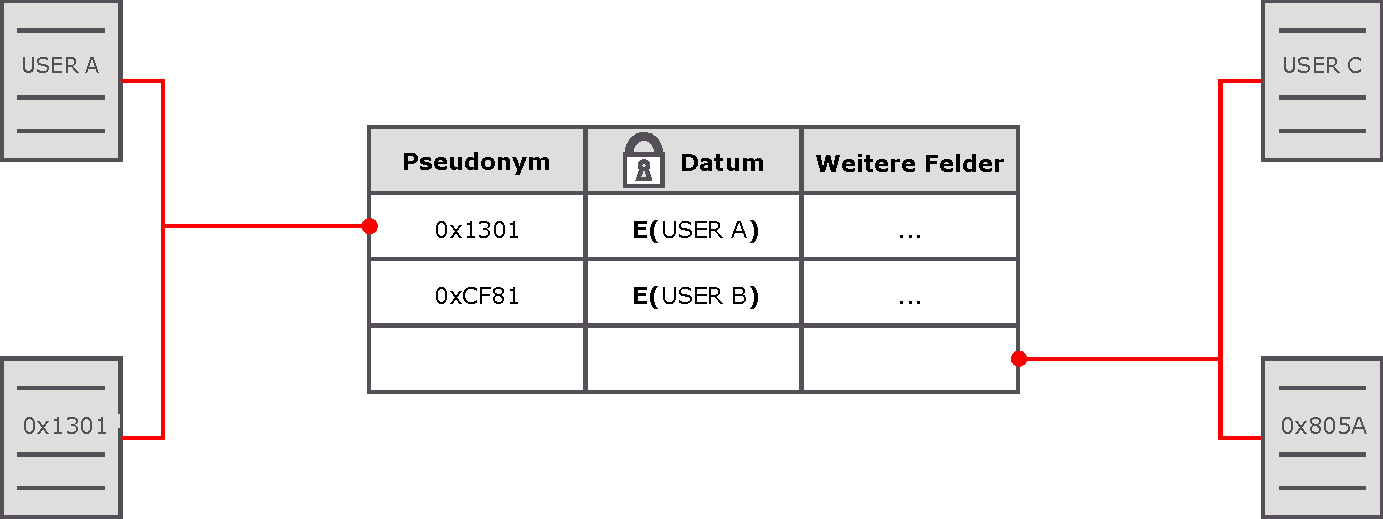
\includegraphics[width=0.9\textwidth]{dia/se_overview.pdf}
    \caption{Erhalt von Pseudonymen aus der Zuordnungstabelle: Links für den Fall eines bereits bekannten Datums (hier Benutzer), rechts für ein unbekanntes Datum.}
    \label{fig:se_overview}
\end{figure}

\subsection{Entschlüsseln aller Datensätze}

Da für die Verschlüsselung ein kryptographisches Schwellwertschema verwendet wird, scheiden zwei triviale Möglichkeiten aus: Das Entschlüsseln aller Datensätze zur Überprüfung wäre nicht nur unter Performance-Gesichtspunkten nicht wünschenswert. Es darf auch nicht möglich sein, da die \textit{Shares} zur Entschlüsselung nicht am Ort der Verschlüsselung vorliegen dürfen. Dies ist eine der Grundannahmen, die der Sicherheit des Systems zugrundeliegen. 

\subsection{Deterministische Verschlüsselung}

Die zweite ausscheidende Möglichkeit wäre das Überprüfen aller Einträge auf Schlüsseltextgleichheit. Bei Gleichheit eines Eintrages könnte das entsprechende Pseudonym zurückgeliefert werden. Hierzu müsste ein deterministisches Verschlüsselungsverfahren genutzt werden, das ein Datum immer auf den gleichen Schlüsseltext abbildet. Diese Möglichkeit scheidet jedoch aus, da es sich bei dem verwendeten Schwellwertschema um ein Public-Key-Verfahren, bei dem bei der Verschlüsselung ein Zufallswert einfließt -- folglich ein nicht-deterministisches Verfahren, handelt.\\
Dieser Nicht-Determinismus ist notwendig, da ansonsten zur Aufdeckung eines Pseudonyms auch ein Wörterbuchangriff mithilfe des öffentlichen Schlüssels des Schwellwertschemas genutzt werden könnte. Ein Angreifer würde alle möglichen Werte, die ein Datum annehmen kann, mit dem öffentlichen Schlüssel verschlüsseln und mit dem aufzudeckenden Eintrag vergleichen. Gleichheit der Schlüsseltexte würde den gesuchten Klartext liefern. Der im Kontext dieser Arbeit vorliegende kleine und bekannte Wertebereich (wie beispielsweise Mitarbeiternamen) würde diesen Angriff relativ effizient machen. Aus diesem Grund muss ein nicht-deterministisches Verschlüsselungsverfahren genutzt werden und damit ist die Überprüfung auf Schlüsseltextgleichheit nicht möglich.


\subsection{Nutzung von Hashfunktionen}

Ein weiterer Ansatz, der ebenfalls anfällig für diese Art von Wörterbuch-Angriff wäre, ist die Verwendung von (kryptographisch sicheren) Hashfunktionen zur Suche: Neben dem Pseudonym und dem verschlüsselten Datum wird ein Hash des Datums abgespeichert. Muss nun für ein neues Datum überprüft werden, ob bereits ein Pseudonym vorliegt, kann der Hash des Datums gebildet und mit allen vorliegenden Hashes verglichen werden. Bei Übereinstimmung wäre das Datum (mit großer Wahrscheinlichkeit) gleich dem verschlüsselten Datum und das Pseudonym könnte genutzt werden. Diese Möglichkeit ist jedoch durch den bereits erwähnten kleinen Wertebereich ebenso anfällig für einen Wörterbuchangriff: Ein Angreifer könnte mithilfe der bekannten Hashfunktion die Hashes aller Werte berechnen und mit dem des aufzudeckenden Pseudonyms vergleichen.

\subsection{Lokale Zuordnung}

Eine andere Möglichkeit ist die Anlage einer vor externem Zugriff geschützten Zuordungstabelle zwischen Datum und Pseudonym am Ort der Ersetzung. Bei Eintreffen eines neuen Datums kann in der Tabelle das zugehörige Pseudonym ermittelt werden oder falls es noch nicht existiert, ein neues Pseudonym erstellt und zusammen mit dem verschlüsselten Datum gespeichert werden. Diese Lösung wirda auch in \cite{goh2003} erwähnt.

Nachteil bezogen auf das für diese Arbeit zu entwickelnde System ist jedoch die notwendige Generierung von Pseudonymen und Speicherung der Zuordnungstabelle an der Stelle, an der neue Daten eintreffen. Hierdurch wird ein relativ leichtgewichtiger Proxy-Server wie er in der Architektur vorhergesehen ist (siehe Abschnitt \ref{sec_impl_architecture}) verhindert. Außerdem würde eine Kompromittierung dieser Komponente direkt zur Aufdeckung des Pseudonymzusammenhanges führen. \todo{Verhindert verteiltes System - diesen Aspekt betonen (mehrere Proxies, ...)}

\subsection{Message Authentication Codes}

Aufbauend auf der Hash-basierten Lösung lässt sich jedoch auch eine nicht für einen Wörterbuchangriff anfällige Lösung entwickeln. Dazu wird der verwendete Hash durch einen schlüsselabhängigen MAC (siehe Abschnitt \ref{sec_mac}) ersetzt. Beim Speichern eines neuen Eintrags wird dazu unter Zuhilfename eines zufällig generierten Schlüssels ein MAC über das Datum berechnet und mit dem Eintrag gespeichert. Für ein Datum kann jetzt durch Überprüfen aller MACs bestimmt werden, ob bereits ein Pseudonym vergeben wurde. Ein Angreifer kann den beschriebenen Wörterbuchangriff jedoch ohne Kenntnis des Schlüssels nicht ausführen.

Bei dieser Lösung handelt es sich um eine einfache Form der Searchable Symmetric Encryption wie sie in Abschnitt \ref{sec_basisc_se} dargestellt ist. Die durch Pseudonyme zu ersetzenden Daten bilden die zu durchsuchenden Dokumente. Der MAC bildet den Suchwort-Index für jeden verschlüsselten Eintrag und wird so auch als Trapdoor-Element für die Suche nach einem passenden Eintrag genutzt. Ausgehend von den Anforderungen des umzusetzenden Systems eignet sich dieser Ansatz: Er ermöglicht einer Komponente die Zuordnung eines Datums zu einem Pseudonym, ohne dass dass diese Zuordnung direkt gespeichert werden muss oder der Datenbank bei der Abfrage bekannt wird. Auch ein Wörterbuchangriff, der bei dem erwähnten kleinen Wertebereich geringen Aufwand bedeutete, wird verhindert. Aus diesen Gründen wird dieser Lösungsansatz in einem späteren Schritt im zu entwickelnden System umgesetzt.

Die Nutzung von deterministischer Verschlüsselung (mit der hier beschriebenen Verwendung eines MACs als Sonderfall) wird erstmals in \cite{bellare2007deterministic} beschrieben. Dort werden auch einige Schwächen dieser Lösung diskutiert: Die Datenbank erfährt durch den Suchindex bereits einiges über die gespeicherten Dokumente, da durch die deterministische Struktur gleiche Suchwörter auf gleiche Trapdoor-Elemente abgebildet werden. Diese Schwäche ist im Bezug auf den besonderen Anwendungsfall dieser Arbeit jedoch zu vernachlässigen, da Dokumente (meint Benutzernamen, ...) nur einmalig vorliegen dürfen. Eine weitere Schwäche, die auch in dieser Arbeit beachtet werden muss, ist, dass die Datenbank etwas über die Häufigkeit verschiedener Suchanfragen erfährt, da die Trapdoor-Elemente für ein bestimmtes Datum immer gleich sind. Durch Korrelation mit Hintergrundwissen könnte so möglicherweise in bestimmten Fällen der Inhaber eines Pseudonyms herausgefunden werden. 
\todo{Hash-Kollisionen und Geburtstags-Paradoxon hier erwähnen?}

\subsection{Weitere Möglichkeiten der Searchable Encryption}
\label{sec_state_se_furtherpossibilities}

%- SongWagner \cite{song2000practical}
%- survey \cite{wang2016}
%- goh \cite{goh2003}
%- chang \cite{chang2005}

Die im letzten Abschnitt betrachtete MAC-basierte Lösung funktioniert für den in dieser Arbeit behandelten Anwendungsfall. Bei der Abbildung Pseudonym zu Datum (wie den Benutzername) handelt es sich um eine 1:1-Abbildung, die lediglich von einer Komponente -- dem zu entwickelnden Log-Proxy -- abgefragt wird. 

In anderen Umgebungen bzw. Erweiterungen des in dieser Arbeit betrachteten Anwendungsfalls kann es jedoch auch andere Anforderungen geben. Vorstellbar wäre beispielsweise die verteilte Abfrage der Datenbank nach existierenden Pseudonymen. Für den MAC-basierten Ansatz müsste dazu zumindest der genutzte Schlüssel verteilt werden, was Kommunikation innerhalb der verteilten abfragenden Komponenten erfordert. Zusätzlich müssten auch die Sicherheitsauswirkungen dieser Lösung betrachtet werden.\\
Eine andere Erweiterung könnte die Mehrfachverwendung von Pseudonymen für verschiedene Merkmale eines Benutzers (Name, IP-Adresse, Signaturschlüssel, ...) sein, um die Erkennung von Insiderangriffen zu verbessern. Auch diese Erweiterung wäre mit dem MAC-basierten Ansatz nicht direkt abbildbar.

Andere Lösungsansätze für die in diesen Fällen entstehenden Probleme könnten Forschungsergebnisse aus dem Bereich der \textit{Searchable Encryption} bieten. In \cite{song2000practical} wurde von den Autoren das erste Searchable-Symmetric-Encryption-Schema entwickelt (siehe auch Abschnitt \ref{sec_basisc_se}). Verbesserte Schemata folgten in \cite{goh2003} und \cite{chang2005}. Durch diese sind variable Dokumentenlängen mit beliebig vielen Suchwörtern möglich, die auch nachträglich erweiterbar sind. Für den Aspekt der verteilten Abfrage könnten die Ergebnisse aus \cite{boneh2004public} genutzt werden, in dem sich die Autoren mit der Suche in mit asymmetrischen Verfahren verschlüsselten Daten befassen.\\
Eine Übersicht über weitere Ergebnisse in diesem Bereich lässt sich in \cite{wang2016} finden.